%!TEX root = /Users/jakubkonka/Thesis/Thesis.tex
\chapter{Direct Analysis of Network Selection Mechanism} % (fold)
\label{cha:direct}

This chapter formally defines the network selection mechanism in the DMP, and casts it into the framework of game theory. The mechanism is then directly analysed in three special cases: 1) when only reputation ratings of the network operators decide on the winning network operator, 2) when only the monetary bids of the network operators matter in the selection of the winner, and finally, 3) when all network operators are characterised by the same reputation rating. In essence, those special cases correspond to the extremes of the studied bidding problem, and in all those cases, the equilibrium bidding strategies are derived. The chapter then concludes with the analysis of the mechanism in a restricted case with only two network operators, for which the equilibrium bidding strategies are derived. They are shown, however, to be suboptimal as they allow the network operators to submit a negative monetary bid.

\section{Problem Definition and Assumptions} % (fold)
\label{sec:problem_definition_and_assumptions_direct}
\annotate{C4.10}{The game-theoretic description of the network selection mechanism employed in the DMP is as follows. The model constitutes a version of procurement first-price sealed-bid auction (henceforth, referred to as FPA). To recap, in FPA, bidders submit their bids simultaneously~\cite{Gibbons92}. Furthermore, each bidder knows their own cost of selling the good to the buyer but does not know any other bidder's type; i.e., the costs are private knowledge. The bidder who submitted the highest bid, wins the auction and sells the good to the buyer for the price equivalent to their bid. Since the costs are private knowledge, the bidders are uncertain about another bidders' utility functions. Thus, FPA and the network selection mechanism represent Bayesian games of incomplete information (see Section~\ref{sec:theory_of_games_notation}, Appendix~\ref{cha:notation} for the formal definition of a Bayesian game of incomplete information).}

There are $n$ network operators who bid for the right to sell their product to the subscriber such that $n = |N|$ where $N$ denotes the set of all network operators. Let $\beta : \mathbb{R}_+\times [0,1] \to \mathbb{R}_+$, defined by
\begin{equation}
	\label{eq:def_beta_direct}
	\beta(b_i, r_i) = w_{price}\cdot b_i + w_{penalty}\cdot r_i \quad\text{for all } i\in N,
\end{equation}
denote the compound bid. Each network operator $i$ is characterised by the utility function $u_i$ such that
\begin{equation}
	\label{eq:sellers_utility_direct}
	u_i(b,c,r) = \left\{
	\begin{array}{l l}
		b_i-c_i & \;\text{if } \beta(b_i, r_i) < \displaystyle\min_{j\neq i}\beta(b_j,r_j),\\
		0 & \;\text{if } \beta(b_i, r_i) > \displaystyle\min_{j\neq i}\beta(b_j,r_j),
	\end{array}\right.
\end{equation}
where $b = (b_i,b_{-i})$ represents the monetary bid (or offered price) vector, $c = (c_i, c_{-i})$ the cost vector, and $r = (r_i, r_{-i})$ the reputation rating vector. \annotate{C4.8}{In this notation, $b_{-i}$ is a shorthand notation for a vector containing all elements with the $b_i$ excluded; that is, $b_{-i} = (b_1, \ldots, b_{i-1}, b_{i+1}, \ldots, b_n)$.} \annotate{C4.9}{Furthermore, as already stated in Section~\ref{sub:conceptual_overview_dmp}, Chapter~\ref{cha:dmp}, the monetary bid is equivalent to the price of supporting the service by the network operator. The precise definition of the price is left open-ended; one possibility, for example, would be to charge the buyer per unit of bandwidth.}

The cost of each network operator is assumed to represent the minimum price for transporting the service request under consideration. The winner of the auction is determined as the network operator whose compound bid is the lowest one; i.e., network operator $i$ is the winner if
\begin{equation}
	\beta(b_i, r_i) < \displaystyle\min_{j\neq i}\beta(b_j,r_j).
\end{equation}
In the event that there is a tie
\begin{equation}
	\beta(b_i, r_i) = \displaystyle\min_{j\neq i}\beta(b_j,r_j),
\end{equation}
the winner is randomly selected with equal probability.

\annotate{C4.6}{It is, moreover, assumed that the price and reputation weights $(w_{price}, w_{penalty})$ are announced by the subscriber to all network operators before the auction. They are specific to the subscriber and the service they requested. In other words, it is envisaged that the same subscriber might use different weights for subsequently requested services during their participation in the DMP.} Since the weights are announced by the subscriber to all network operators before the auction, there is no uncertainty in knowing how much the subscriber values the offered price of the service over the reputation of the network operator (or vice versa). Furthermore,
\begin{equation}
	w_{price} + w_{penalty} = 1,\quad 0\le w_{price},w_{penalty} \le 1.
\end{equation}
In order to simplify the notation, it is assumed throughout the rest of this thesis that $w=w_{price}$. This simplifies the definition of the compound bid in Equation~\eqref{eq:def_beta_direct} to
\begin{equation}
  \beta(b_i, r_i) = wb_i + (1-w)r_i\quad\text{for all } i\in N.
\end{equation}
Note, however, that since $w$ is assumed to be common knowledge, it could potentially lead to a situation where network operators manipulate the knowledge of $w$ to increase their profits by overcharging the subscriber. Therefore, in order to circumvent such an eventuality, the subscriber would only consider offers such that
\begin{equation}
	\label{eq:subscribers_valuation_direct}
	v\geq wb_i + (1-w)r_i \quad\text{for all } i\in N
\end{equation}
where $v\in (0,1]$ is the subscriber's valuation, and it is private knowledge~\cite{DMLeBodic00}. The subscriber's valuation is effectively equivalent to a secret (or hidden) reserve price~\cite{Vincent1995575,LiPerrigne1999,BajariHortacsu2003}. This creates an additional uncertainty about the auction that each network operator needs to incorporate into their equilibrium bidding strategies. To elaborate further, by setting a secret reserve valuation, the subscriber creates a phantom bidder characterised by a reputation rating $r_0$ and submitting a bid $b_0$ such that $v=\beta(b_0,r_0)$, and therefore, risks not obtaining a service offer from any network operator if $v < \beta(b_i,r_i)$ for all $i\in N$. Therefore, the solution presented in this and the following chapters would have to be modified by including the phantom bidder in the derivation of the equilibrium bidding strategies. However, in order to keep the analysis tractable, this assumption is not incorporated in this research.
	
Following the standard assumptions from the auction literature~\cite{Krishna10}, the set of network operators, $N$, is finite and the network operators are risk neutral; that is, they seek to maximise their expected profits. Furthermore, the subscriber is risk neutral and does not have any budget constraints; that is, the subscriber is prepared to accept any offer from the network operators. In reality, it is unlikely for the network operators and the buyer to be risk neutral, and the buyer to not have any budget constraints. However, in order for the problem to be tractable, those assumptions are enforced in this research. The implications of relaxing those assumptions on the analysis of an auction are explored by Krishna~\cite{Krishna10}.

The costs $c_i$ for each network operator $i$ are private knowledge. Thus, they are particular realisations of the random variables (r.v.) $C_i$ for each $i$. Furthermore, it is assumed that each $C_i$ is identically and independently distributed (i.i.d.) over the interval $[0,1]$ according to some (absolutely-) continuous probability distribution which admits a distribution function $F_{C}$ and an associated density function $f_{C}$ such that $f_C$ is locally bounded away from zero over the interval $[0,1]$. In order to keep the specification generic, the costs are not explicitly decomposed into the underlying components such as interconnection charges, infrastructure fixed costs, etc. The reader is referred to~\cite{Njoroge2009,LeCadre2009,HauBrenner2009} for an in-depth coverage of the problem. Furthermore, it is recognised that various network operators will have different architecture, topology, infrastructure, etc., and that this impacts cost to support the service. In order to capture the variation in costs, an i.i.d.~random variable is employed to assign a cost to a particular network operator at the time of the service request. This further aids generality of the results and subsequent analysis presented in this research.

The reputation ratings $r_i$ for each network operator $i$ are common knowledge. It is assumed that each $r_i\in [0,1]$ such that the higher the reputation, the lower the rating $r_i$. Initially, it was assumed that ratings are private knowledge. However, after analysis, it was concluded that this would contradict its purpose. The reputation of each network operator, in order to be meaningful, must be freely available to everyone, including the competitors of the network operators. For example, in the Amazon.com Marketplace, the buyers have the right to rate the seller they buy from on a scale from one to five (with five being the best), and these ratings are publicly available~\cite{AMAZON}. Similarly, on eBay, the buyers can leave sellers feedback (negative, neutral, or positive) which over time is viewed as reputation, and is also publicly available~\cite{EBAY}.
	
The bidding strategy functions $b_i: [0,1]\to\mathbb{R_+}$ are nonnegative in value for all $i$. The aim is to solve the game for pure-strategy Bayesian Nash equilibrium(-a) as defined in Equation~\eqref{eq:def_bayesian_nash_eq_notation}, Section~\ref{sub:static_games_with_incomplete_information_notation}, Appendix~\ref{cha:notation}. \annotate{C4.7}{It is further assumed that the network operators will bid at least their cost (unless explicitly stated otherwise). The problem of bidding below cost or negatively deserves a more elaborate explanation. There are two fundamental assumptions governing game theory~\cite{Myerson97}: 1) economic agents are rational decision-makers; that is, they make decisions consistently in pursuit of their own objectives; and 2) their objective is to maximise the expected value of their own utility. In the light of those assumptions, network operators are implied to bid at least their cost as they would always strive to maximise their expected utility. However, the real behaviour of the network operators might be different in the sense that they might, in the view of game theory, behave irrationally by bidding below their cost to secure the contract with the subscriber. In fact, if the temporal aspect of the DMP is considered, network operators will interact by engaging in the DMP auction more than once. Then, it might prove beneficial for them to bid below their cost trading positive utility for securing the win---this is a well-known pricing strategy in economics called ``loss leader'' pricing strategy~\cite{DeGraba2006,In2014}. The idea behind the strategy is to sell a good at a price below its market cost to increase the store traffic and encourage sales of other, possibly more profitable goods. Applied back to the DMP, a network operator could, in principle, willingly incur cost by bidding below their cost to encourage more subscribers to use their services, or to improve their reputation rating by serving more subscribers. While the fact that situations like this can occur in reality is appreciated, this thesis follows the fundamental assumptions of game theory; that is, in the rest of this thesis (unless explicitly stated otherwise), it is assumed that all economic agents involved in the DMP are rational decision-makers and strive to maximise their expected utility. Otherwise, the mathematical treatment of the problem would prove impossible~\cite{VonNeumann2004}.}

The problem is divided into two cases: generic and restricted case. In the former case, no additional assumptions about the game than those already stated in this section will be made, and the discussion will concentrate on finding a symmetric equilibrium. In the latter case, on the other hand, the problem will be simplified by considering only two network operators, letting costs be drawn from the uniform distribution, and focusing on (possibly different) bidding strategy functions which are linear functions of cost.
% section problem_definition_and_assumptions (end)

\section{Generic Case} % (fold)
\label{sec:direct_generic_case_direct}
Suppose that all network operators use the same strictly increasing in $c_i$ bidding strategy function; i.e., $b_i = b_i(c_i) = b(c_i)$ for all $i\in N$. In this case, the equilibrium profile $(b^*,\ldots,b^*)$ is called \emph{symmetric}. In its generic form, the problem proves to be too complicated for the analytical solution using the existing methods of solving auctions. It would seem that since the problem is a modified version of the standard FPA, the standard analytical approach, found for example in~\cite{Krishna10,McAfee1987,Hansen88,Dastidar08}, should apply. However, this is not the case. To see why, note that each network operator $i$ faces an optimisation problem
\begin{equation}
	\label{eq:simple_foc_direct}
	\max_{b_i}E\left[ b_i-c_i \:\middle\vert\: wb_i + (1-w)r_i < \displaystyle\min_{j\neq i}(wb(C_j) + (1-w)r_j) \right].
\end{equation}
Note that
\begin{equation}
	\label{eq:overestimation_direct}
	\displaystyle\min_{j\neq i}(wb(C_j) + (1-w)r_j) \ge w\displaystyle\min_{j\neq i}b(C_j) + (1-w)\displaystyle\min_{j\neq i}r_j.
\end{equation}
Substituting the inequality~\eqref{eq:overestimation_direct} into the identity~\eqref{eq:simple_foc_direct}, yields for all $w\neq 0$
\begin{equation}
	\max_{b_i}E\left[ b_i-c_i \:\middle\vert\: b^{-1}\left(b_i + \frac{1-w}{w}(r_i-\displaystyle\min_{j\neq i}r_j)\right) < \displaystyle\min_{j\neq i}C_j \right],
	\label{eq:ode_part1_direct}
\end{equation}
where the fact that $b$ is increasing was used, and hence, it is invertible (cf.~Corollary~\ref{cor:increasing_invertible_notation}) and $\min_{x}b(x) = b(\min_{x}x)$ for all $x$.

Let $C_{1:n-1} = \min_{j\neq i}C_j$ be the lowest order statistic of an i.i.d.~random sample $C_j$ for all $j\neq i$ with the distribution function $F_{C_{1:n-1}}$. Hence, the identity~\eqref{eq:ode_part1_direct} becomes
\begin{align}
	&\max_{b_i}\bigg(b_i-c_i\bigg)\left(1 - F_{C_{1:n-1}}\left(b^{-1}\left(b_i + \frac{1-w}{w}(r_i-\min_{j\neq i}r_j)\right)\right)\right) \nonumber\\
	= &\max_{b_i}\bigg(b_i-c_i\bigg)\left(1 - F_{C}\left(b^{-1}\left(b_i + \frac{1-w}{w}(r_i-\min_{j\neq i}r_j)\right)\right)\right)^{n-1},
	\label{eq:ode_part2_direct}
\end{align}
where the fact was used that the distribution function of an $i^\textrm{th}$ order statistic of an i.i.d.~random sample is defined as in Equation~\eqref{eq:iid_cdf_notation}, Section~\ref{sub:order_statistics_notation}, Appendix~\ref{cha:notation}.

Finally, recalling that at a symmetric equilibrium $b_i=b(c_i)$ and letting $k=\nobreak\frac{(1-w)}{w}(r_i-\min_{j\neq i}r_j)$, the identity~\eqref{eq:ode_part2_direct} becomes
\begin{align}
	\label{eq:ode_final_form_direct}
	&\frac{d}{dc_i}b\left( b^{-1}(b(c_i) + k) \right) \left[ 1 - F_C(b^{-1}(b(c_i)+k)) \right]^{n-1} \nonumber\\
	= &(n-1)(b(c_i)-c_i)\left[ 1 - F_C(b^{-1}(b(c_i)+k)) \right]^{n-2} f_C(b^{-1}(b(c_i)+k)).
\end{align}
It is difficult (if possible) to derive a closed-form solution for the resulting ordinary differential equation in Equation~\eqref{eq:ode_final_form_direct}. Therefore, it can be concluded that even significant simplification of the problem is not enough to heuristically derive an optimal bidding strategy function for each network operator $i$. It is possible, however, to derive the optimal bidding strategies in a handful of special cases: $w=0$, $w=1$, and $r_i=r_j$ for all $i,j\in N$ such that $i\neq j$. This is the subject of the next three sections.

\subsection{Special Case $w=0$} % (fold)
\label{sub:special_case_w_0_direct}
In one of the extreme cases, however, when $w=0$, the problem becomes simpler. For then, the utility function simplifies to
\begin{equation}
	\label{eq:utility_w_0_direct}
	u_i(b,c,r) = \left\{
	\begin{array}{l l}
		b_i-c_i &\text{if } r_i < \displaystyle\min_{j\neq i} r_j,\\
		0 &\text{if } r_i > \displaystyle\min_{j\neq i} r_j.
	\end{array}\right.
\end{equation}
Since the reputation ratings, $r_i$, are common knowledge, the probability of winning, i.e., the probability of the event such that $r_i<\min_{j\neq i}r_j$ for all $i$, is either $0$ or $1$, and does not depend on the value of the bid, $b_i$. In other words, each network operator knows in advance whether they won, tied, or lost based on their own and their opponents reputation ratings since these are deterministic in nature. Hence, it is clear that the network operator with the lowest reputation rating will have an incentive to bid abnormally high since they are guaranteed a win regardless of the value of their bid. The remaining network operators, on the other hand, will be indifferent to the value of the submitted bids as it is impossible for them to win regardless of the values of their bids. In case of a tie, i.e., in case there is more than one network operator with the lowest reputation rating, each has an equal probability of winning the auction, and this probability is independent of the values of their bids. Hence, in this case, the network operators also have an incentive to bid abnormally high. Formally,
\begin{proposition}
\label{prop:special_case_w_0_direct}
Suppose $c_i$ is i.i.d.~over the interval $[0,1]$ for all $i\in N$ and $r_i\in [0,1]$ for all $i\in N$ is common knowledge. Let $N_0\subseteq N$ be the set of all those network operators with the lowest reputation rating. If $w=0$, then every network operator $j\in N_0$ will have an incentive to bid abnormally high, i.e., $b_j\rightarrow\infty$, while every remaining network operator $k\in N\setminus N_0$ will be indifferent to the value of their bid.
\end{proposition}
\annotate{G3}{\noindent The formal proof of Proposition~\ref{prop:special_case_w_0_direct} as well as any other proposition included in this thesis is given in Appendix~\ref{cha:proofs}.}
% subsection special_case_w_0_ (end)

\subsection{Special Case $w=1$} % (fold)
\label{sub:special_case_w_1__direct}
When $w=1$, on the other hand, the problem becomes that of standard FPA auction. The utility of each network operator $i$ becomes
\begin{equation}
	\label{eq:sellers_utility_w_1_direct}
	u_i(b,c,r) = \left\{
	\begin{array}{l l}
		b_i-c_i & \quad\text{if } b_i < \displaystyle\min_{j\neq i}b_j,\\
		0 & \quad\text{if } b_i > \displaystyle\min_{j\neq i}b_j.
	\end{array}\right.
\end{equation}
Network operator $i$ conjecturing that other network operators follow $b$ symmetric bidding strategy and submit their costs truthfully, tries to solve
\begin{align}
	\label{eq:standard_fpa_ode_part_1_direct}
	&\max_{b_i}E \left[ b_i-c_i \:\middle\vert\: b_i < \min_{j\neq i}b(C_j) \right] \nonumber\\
	= &\max_{b_i}E \left[ b_i-c_i \:\middle\vert\: b^{-1}(b_i) < \min_{j\neq i}C_j \right] \nonumber\\
	= &\max_{b_i}E \left[ b_i-c_i \:\middle\vert\: b^{-1}(b_i) < C_{1:n-1} \right] \nonumber\\
	= &\max_{b_i} \int_{b^{-1}(b_i)}^{1} (b_i-c_i)dF_{C_{1:n-1}}(t) \nonumber\\
	= &\max_{b_i} (b_i-c_i)(1 - F_{C_{1:n-1}}(b^{-1}(b_i))),
\end{align}
where, as before, $C_{1:n-1} = \min_{j\neq i}C_j$ is the lowest order statistic of an i.i.d.~random sample $C_j$ for all $j\neq i$ with the distribution function $F_{C_{1:n-1}}$, and associated density $f_{C_{1:n-1}}$. The first-order condition yields
\begin{equation}
	\label{eq:standard_fpa_ode_part_2_direct}
	1 - F_{C_{1:n-1}}(b^{-1}(b_i)) - (b_i - c_i)\frac{f_{C_{1:n-1}}(b^{-1}(b_i))}{\frac{d}{db_i}b(b^{-1}(b_i))} = 0.
\end{equation}
Recalling that at a symmetric equilibrium $b_i=b(c_i)$, the identity \eqref{eq:standard_fpa_ode_part_2_direct} becomes
\begin{equation}
	\label{eq:standard_fpa_ode_part_3_direct}
	\frac{d}{dc_i}b(c_i) - b(c_i)\frac{f_{C_{1:n-1}}(c_i)}{1 - F_{C_{1:n-1}}(c_i)} = -c_i \frac{f_{C_{1:n-1}}(c_i)}{1 - F_{C_{1:n-1}}(c_i)},
\end{equation}
or equivalently,
\begin{equation}
	\frac{d}{dc_i}(b(c_i)(1 - F_{C_{1:n-1}}(c_i))) = -c_if_{C_{1:n-1}}(c_i).
\end{equation}
\annotate{C4.5}{Since $c_i\in [0,1]$ for all $i\in N$, it follows $b(1) = 1$. To see this, suppose network operator 1 is characterised by cost $c_1 = 1$. Then, they would never submit a bid higher than their cost $c_1 = 1$ since they would never win. That is, the competing network operator, network operator 2 say, regardless of their cost, could just bid $b(c_2) = c_1 = 1$ and win the auction. Furthermore, network operator 1 would never submit a bid lower than their cost $c_1 = 1$ since they would make a loss if they were to win the auction. Therefore, it must be that $b(1) = 1$.} It follows then
\begin{align}
	\label{eq:standard_fpa_ode_solution_direct}
	b(c_i) &= \frac{1}{1 - F_{C_{1:n-1}}(c_i)}\int_{c_i}^{1} tdF_{C_{1:n-1}}(t) \nonumber\\
	&= \frac{n-1}{(1 - F_{C}(c_i))^{n-1}}\int_{c_i}^1 t(1-F_C(t))^{n-2}f_C(t)dt.
\end{align}
Thus, the symmetric bidding strategy in Equation~\eqref{eq:standard_fpa_ode_solution_direct} is the most likely candidate for a symmetric pure-strategy Bayesian Nash equilibrium at $w=1$.
\begin{proposition}
\label{prop:special_case_w_1_direct}
Suppose $c_i$ is i.i.d.~over the interval $[0,1]$ for all $i\in N$ and $r_i \in [0,1]$ for all $i\in N$ is common knowledge. If $w=1$, then the symmetric equilibrium bidding strategy function of the standard procurement first-price sealed-bid auction,
\begin{equation}
	\label{eq:standard_fpa_direct}
	b^*_{FPA}(c_i) = \frac{1}{1 - F_{C_{1:n-1}}(c_i)}\int_{c_i}^{1} tdF_{C_{1:n-1}}(t) \quad\text{for all } i\in N,
\end{equation}
constitutes a symmetric pure-strategy Bayesian Nash equilibrium of the DMP variant of a procurement first-price sealed-bid auction.
\end{proposition}
% subsection special_case_w_1_ (end)

\subsection{Special Case $r_i=r_j$} % (fold)
\label{sub:special_case_r_i_r_j_direct}
In the last extreme case, when all network operators are characterised by the same reputation rating, i.e., when $r_i = r_j$ for all $i\neq j$, and when $w\neq 0$, it can be easily verified that the problem simplifies to the special case $w=1$. To see why, let $r = r_i,$ for all network operators $i$. Then, for all $i\in N$ and $w\neq 0$
\begin{align}
	&\beta(b_i, r) < \min_{j\neq i} \beta(b_j, r)\\\nonumber
	\iff &\frac{1}{w} \left(b_i + \frac{1-w}{w} r\right) < \frac{1}{w} \min_{j\neq i} \left(b_j + \frac{1-w}{w} r\right)\\\nonumber
	\iff &b_i + \frac{1-w}{w} r < \min_{j\neq i} b_j + \frac{1-w}{w} r\\\nonumber
	\iff &b_i < \min_{j\neq i} b_j.
\end{align}
Hence, the utility of each network operator $i$ simplifies to
\begin{equation}
	u_i(b,c,r) = \left\{
	\begin{array}{l l}
		b_i - c_i &\text{ if } b_i < \displaystyle\min_{j\neq i} b_j,\\
		0 &\text{ if } b_i > \displaystyle\min_{j\neq i} b_j.
	\end{array}
	\right.
\end{equation}
Formally,
\begin{corollary}
\label{cor:special_case_r_i_r_j_direct}
Suppose $c_i$ is i.i.d.~over the interval $[0,1]$ for all $i\in N$ and $r_i\in [0,1]$ for all $i\in N$ is common knowledge. Suppose $r_i = r_j$ for all $i\neq j$, and $w\neq 0$. Then, the problem simplifies to the special case $w=1$, and hence, $b^*_{FPA}$ is the symmetric equilibrium bidding strategy (Proposition~\ref{prop:special_case_w_1_direct}).
\end{corollary}

In this section, it was shown that, in the generic case, it is difficult to derive a closed-form solution to the bidding problem. Furthermore, the optimal bidding strategy was characterised in three special cases: $w=0$, $w=1$, $r_i=r_j$ for all $i,j\in N$ such that $i\neq j$.

The problem is considerably simplified by restricting the number of network operators to $n=2$, and letting the costs be drawn from the uniform distribution. In this case, it is possible to derive bidding strategies for both bidders, and this is the subject of the following section.
% subsection special_case_r_i_r_j_ (end)
% section generic_case (end)

\section{Restricted Case $n=2$} % (fold)
\label{sec:direct_restricted_case_n_2_direct}
In this section, the discussion will be restricted to only two network operators. Since the problem in its generic form proved analytically intractable to be solved analytically, this section will explore whether in a much simplified scenario it is possible to find a closed-form solution. To this end, let $n=2$. The utility function for each network operator $i\in \{1, 2\}$ thus becomes
\begin{equation}
	\label{eq:utility_n_2_direct}
	u_i(b,c,r) = \left\{
	\begin{array}{l l}
		b_i - c_i &\text{if } \beta(b_i,r_i) < \beta(b_j,r_j),\\
		\frac{1}{2}(b_i - c_i) &\text{if } \beta(b_i,r_i) = \beta(b_j,r_j),\\
		0 &\text{otherwise}.
	\end{array}\right.
\end{equation}
Furthermore, the assumption concerning the symmetric equilibrium profile is relaxed; that is, network operators are permitted to use differing bidding strategies.

The analysis is conducted in two steps. Firstly, it is assumed that information is complete; that is, that each network operator not only knows their own cost and reputation, but also those of their opponent's. Secondly, the standard case is considered; that is, that the reputation ratings of the network operators are assumed to be known, while the costs are private knowledge.

\subsection{Complete Information} % (fold)
\label{sub:complete_information_n_2_direct}
Here, it is assumed that information is complete; i.e., that each network operator knows their own and their opponent's cost and reputation rating. In total, there are 7 different bidding scenarios to consider as described below.

\begin{figure}[p!]
	\vspace{0.5cm}
	\begin{subfigure}[b]{0.5\textwidth}
	  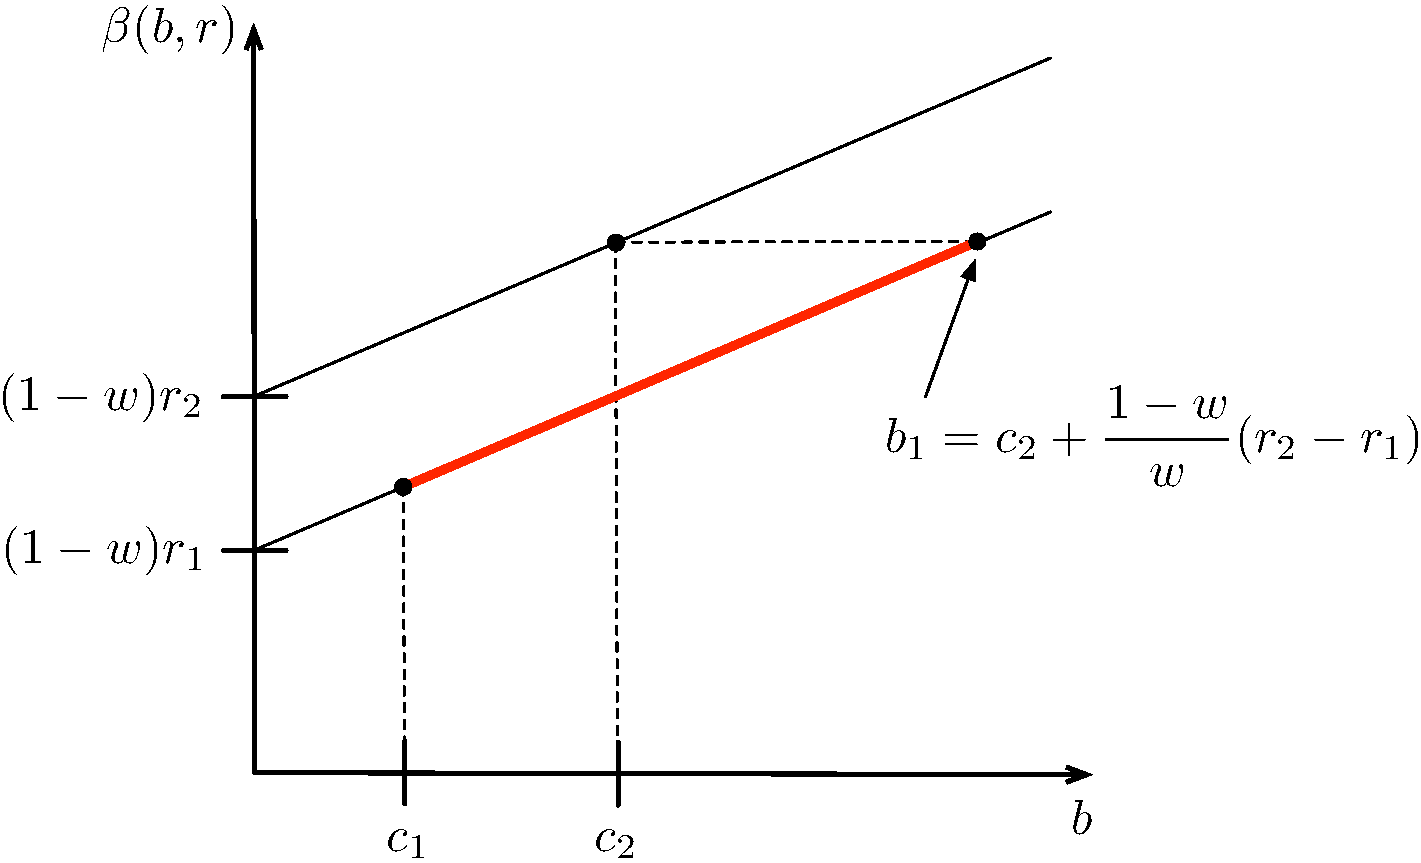
\includegraphics[width=2.8in]{Direct/Figures/complete_N_2_c1}
	  \caption{$c_1 < c_2$}
	  \label{fig:complete_N_2_c1_direct}
	\end{subfigure}
	\begin{subfigure}[b]{0.5\textwidth}
	  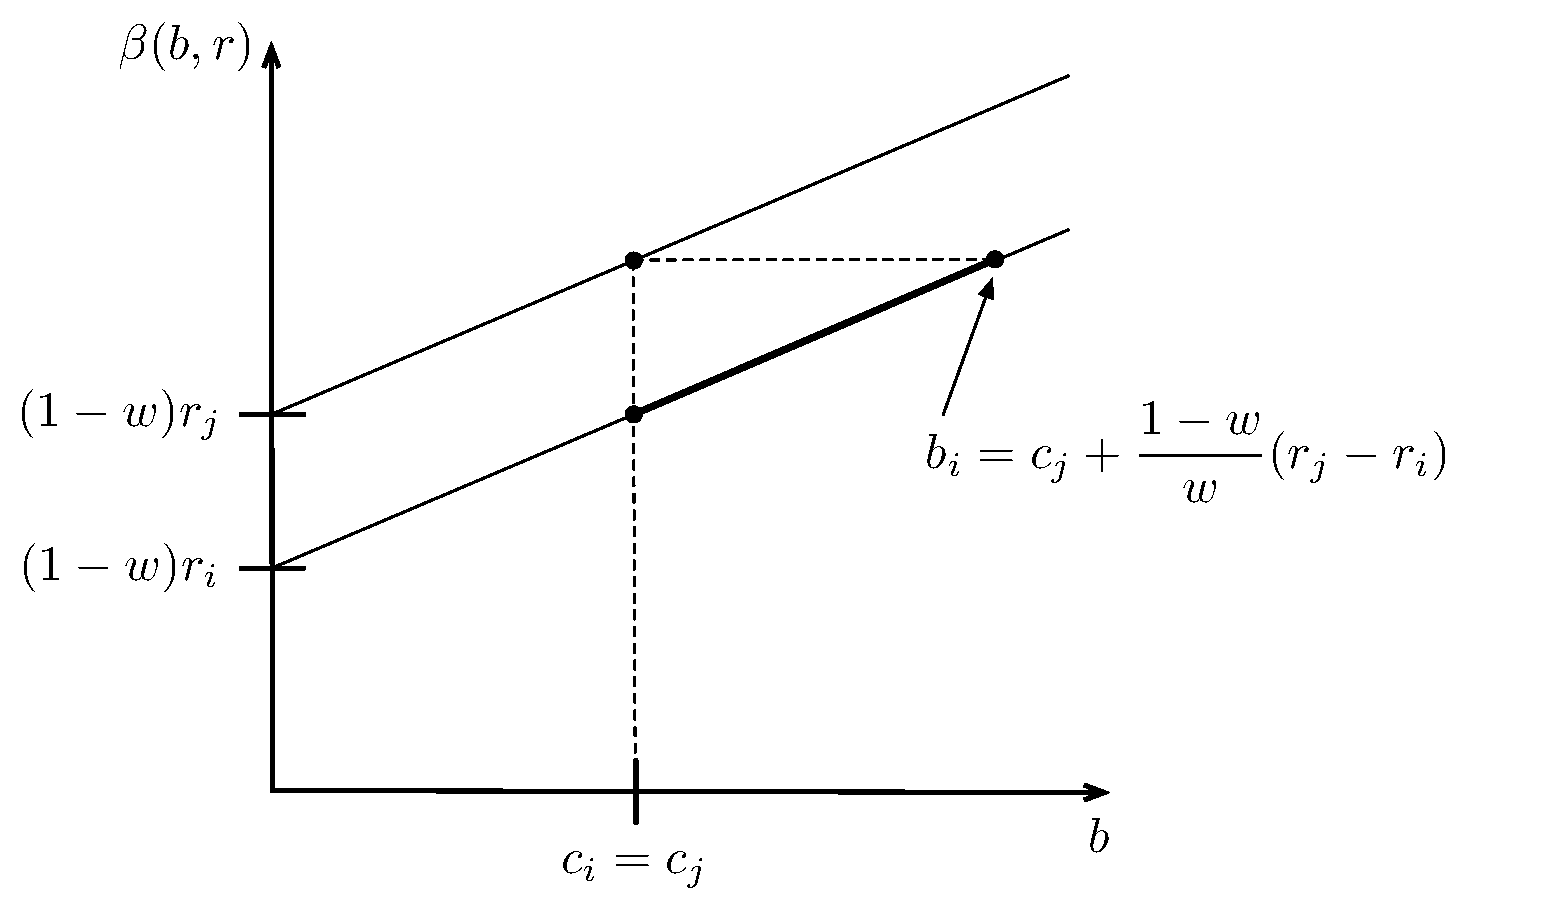
\includegraphics[width=2.8in]{Direct/Figures/complete_N_2_c2}
	  \caption{$c_1 = c_2$}
	  \label{fig:complete_N_2_c2_direct}
	\end{subfigure}
	\vspace{0.5cm}\\
	\begin{subfigure}[b]{0.5\textwidth}
	  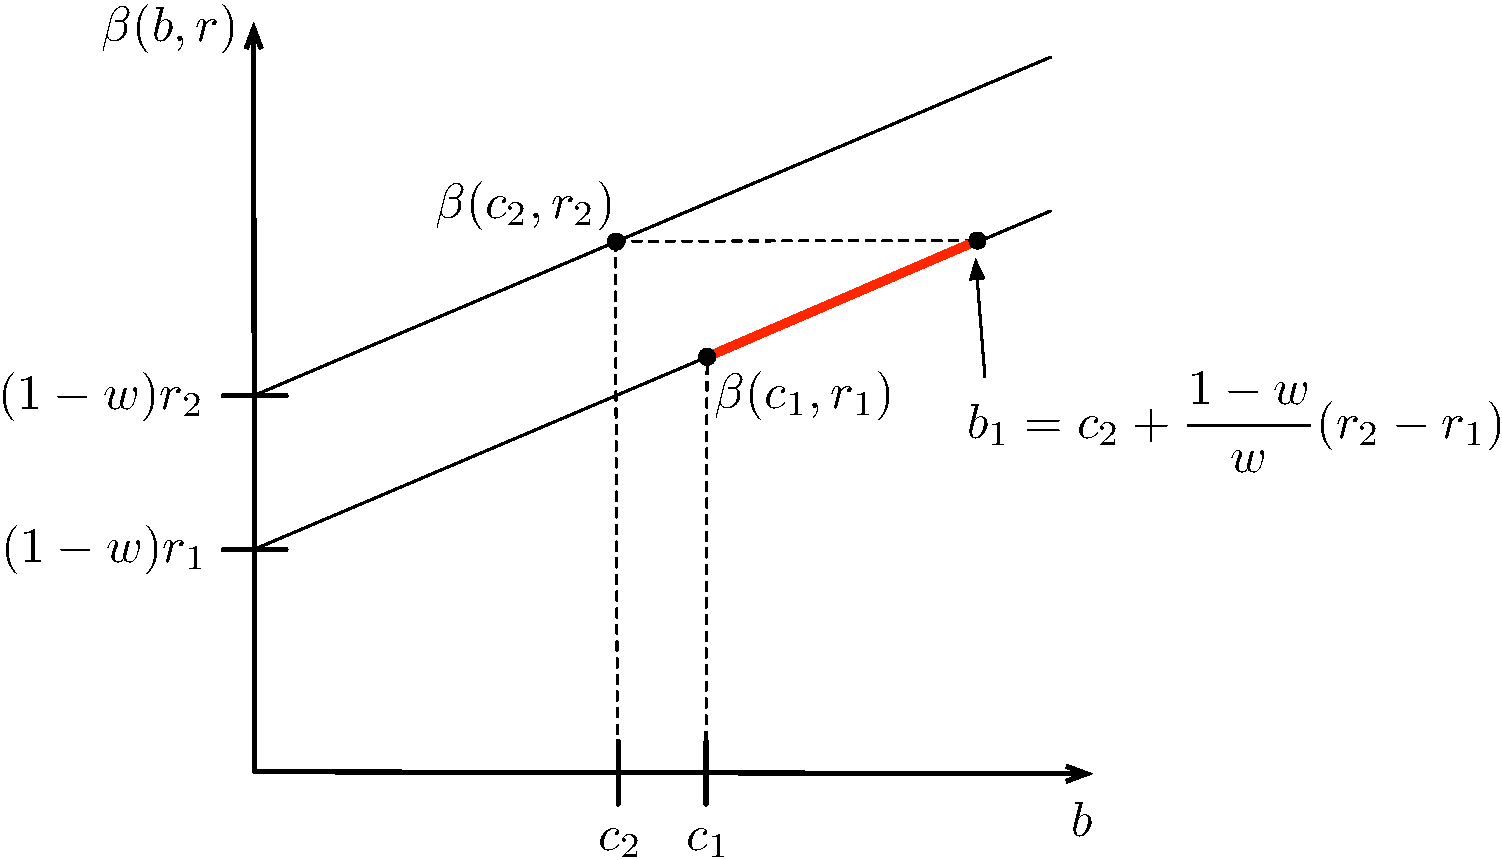
\includegraphics[width=2.8in]{Direct/Figures/complete_N_2_c3_1}
	  \caption{$c_1 > c_2$ and $\beta(c_1,r_1) < \beta(c_2,r_2)$}
	  \label{fig:complete_N_2_c3_1_direct}
	\end{subfigure}
	\begin{subfigure}[b]{0.5\textwidth}
	  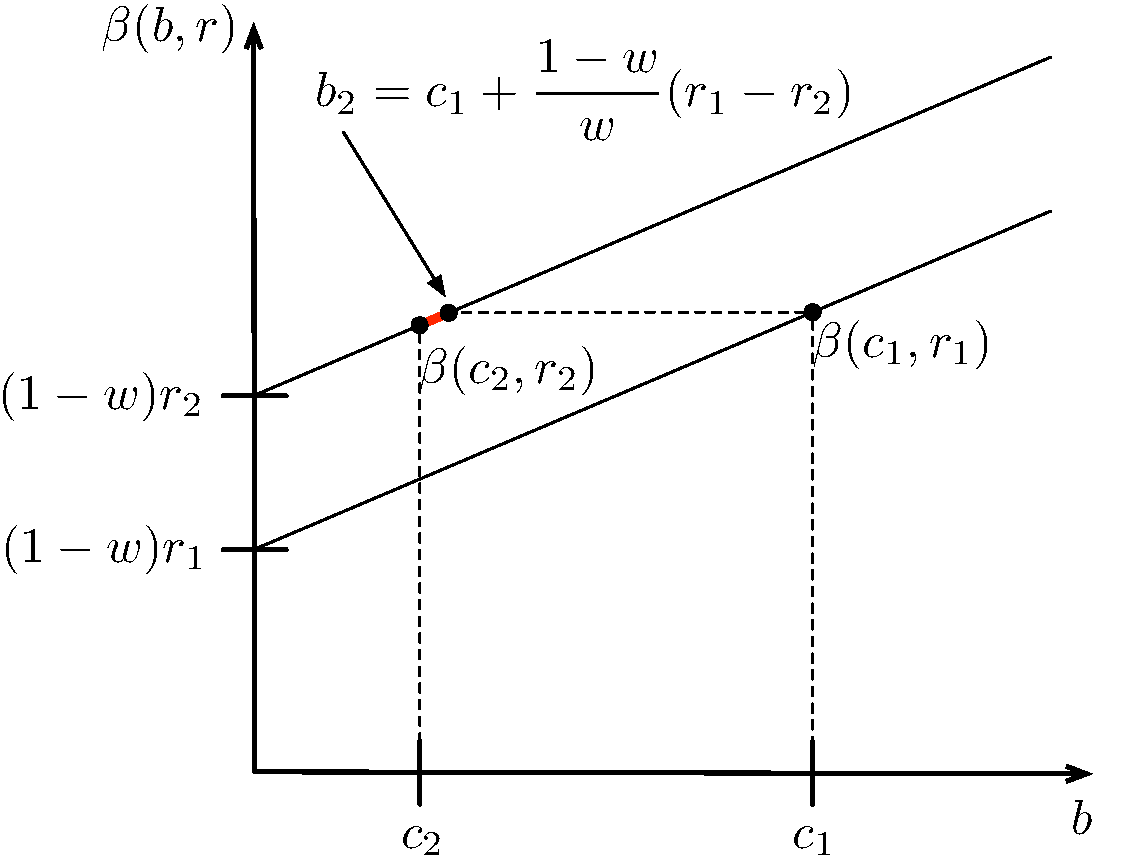
\includegraphics[width=2.8in]{Direct/Figures/complete_N_2_c3_2}
	  \caption{$c_1 > c_2$ and $\beta(c_1,r_1) \ge \beta(c_2,r_2)$}
	  \label{fig:complete_N_2_c3_2_direct}
	\end{subfigure}
	\caption{Different bidding scenarios for $r_1 < r_2$}
	\label{fig:complete_N_2_1_direct}
\end{figure}

\begin{figure}[p!]
	\vspace{0.5cm}
	\begin{subfigure}[b]{0.5\textwidth}
		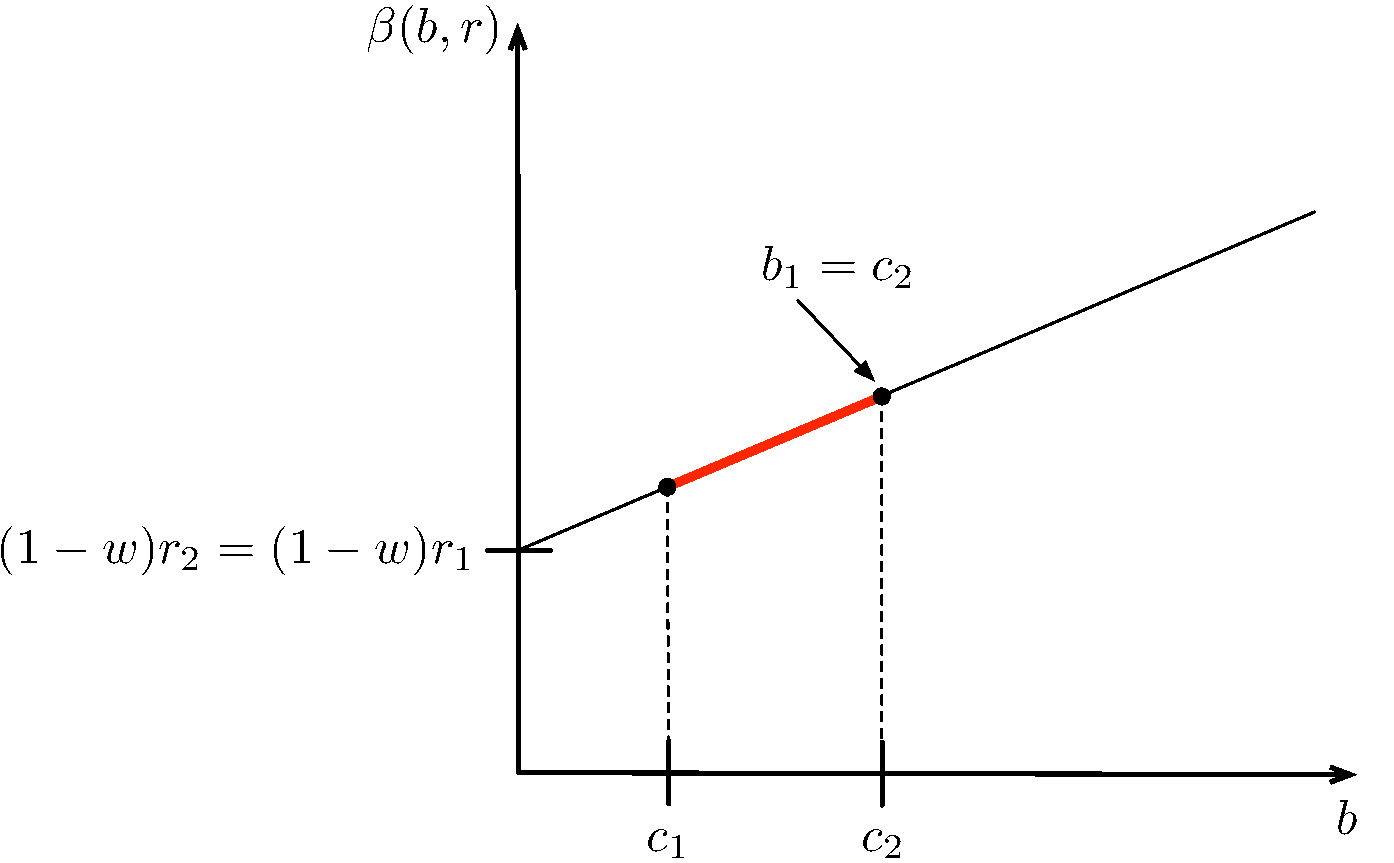
\includegraphics[width=2.8in]{Direct/Figures/complete_N_2_c4}	  
	  \caption{$c_1<c_2$}
	  \label{fig:complete_N_2_c4_direct}
	\end{subfigure}
	\vspace{0.5cm}\\
	\begin{subfigure}[b]{0.5\textwidth}
	  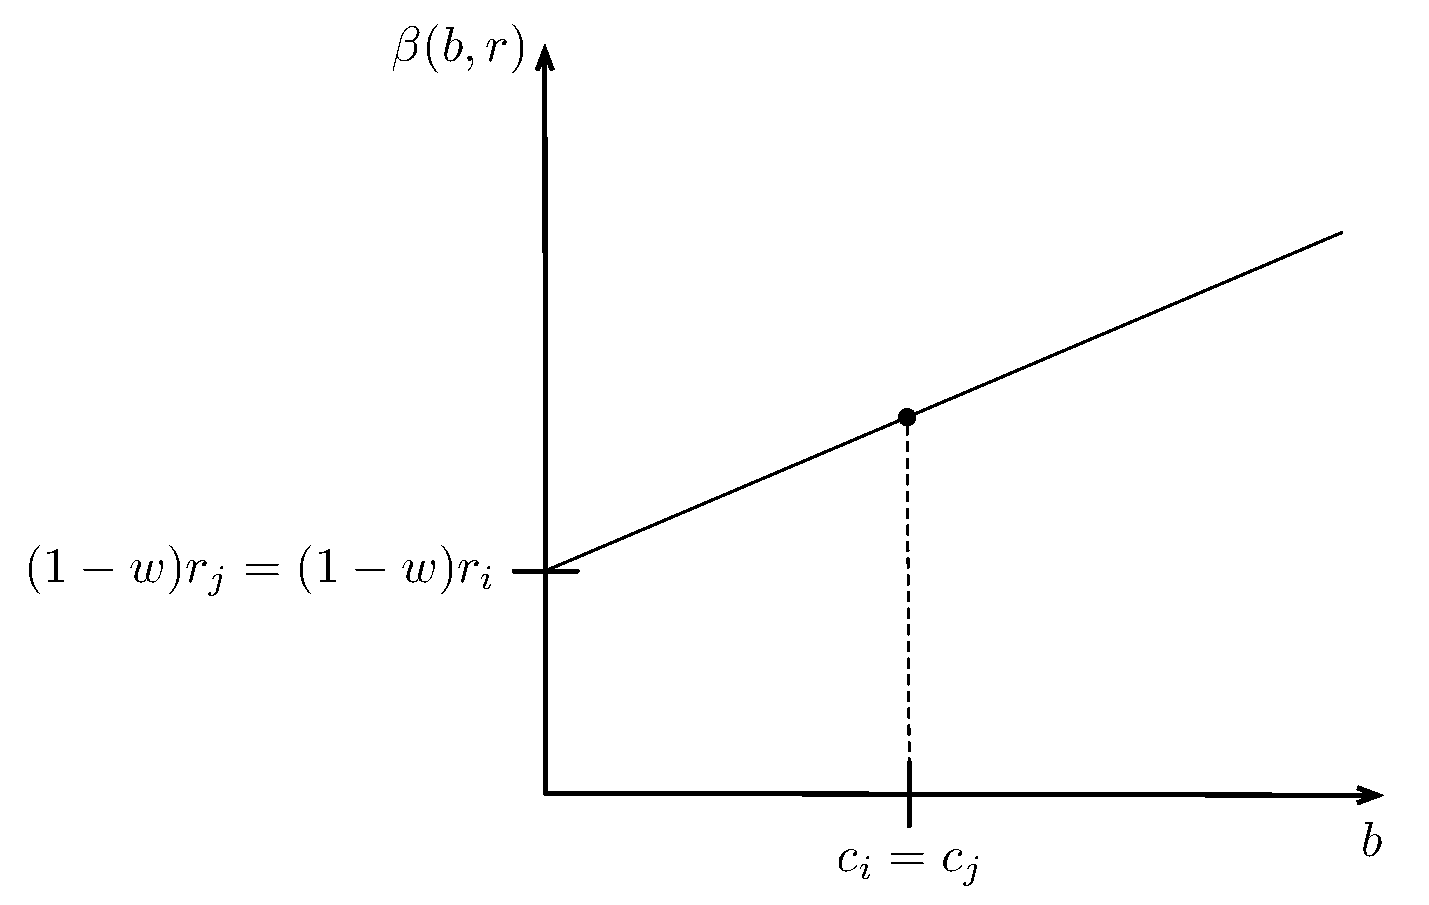
\includegraphics[width=2.8in]{Direct/Figures/complete_N_2_c5}
	  \caption{$c_1=c_2$}
	  \label{fig:complete_N_2_c5_direct}
	\end{subfigure}
	\vspace{0.5cm}\\
	\begin{subfigure}[b]{0.5\textwidth}
	  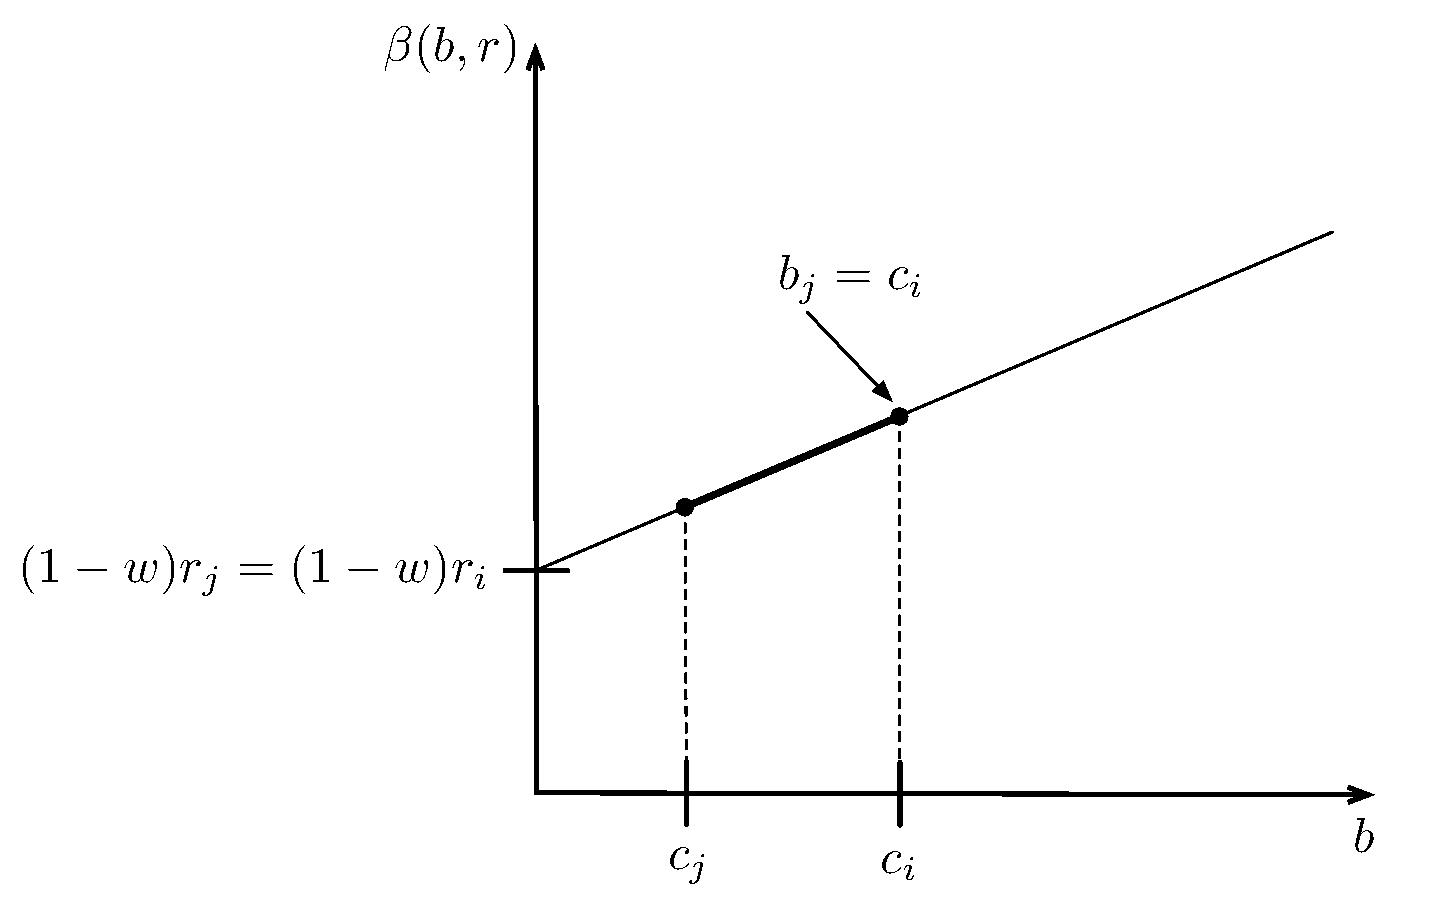
\includegraphics[width=2.8in]{Direct/Figures/complete_N_2_c6}
	  \caption{$c_1 > c_2$}
	  \label{fig:complete_N_2_c6_direct}
	\end{subfigure}
	\caption{Different bidding scenarios for $r_1 = r_2$}
	\label{fig:complete_N_2_2_direct}
\end{figure}

Figure~\ref{fig:complete_N_2_1_direct} shows the first 4 cases for which $r_1 < r_2$. (Note that exactly the same reasoning applies to the situation when $r_1 > r_2$.) If $c_1 < c_2$, network operator 1 is guaranteed a victory and a positive profit as long as they bid within the highlighted part of the $\beta(b,r)$ curve depicted in Figure~\ref{fig:complete_N_2_c1_direct}. Thus, their optimal bidding strategy would be to bid slightly less than their opponent's compound bid evaluated at their opponent's cost, $\beta(c_2,r_2)$; that is, $b_1 = c_2 + \frac{1-w}{w}(r_2-r_1) - \epsilon$ where $\epsilon>0$ is very small. Network operator 2, on the other hand, should find it optimal to bid $b_2 = c_2$. To see why, suppose network operator 2 bids $\hat{b}_2>c_2$. Since network operator 1's reputation rating and cost are strictly lower than those of network operator 2's, they can undercut the network operator 2's bid by a small amount so that $\hat{b}_1 < \hat{b}_2$ and still make positive profit. But, in response, network operator 2 will find it optimal to lower their bid so that it undercuts that of network operator 1's; that is, $\hat{b}_2 < \hat{b}_1$. This process will continue until one of the network operators is forced to bid their cost. Since network operator 1's reputation rating and cost are strictly lower than those of network operator 2's, it can be concluded that $b_2 = c_2$ and $b_1 = c_2 + \frac{1-w}{w}(r_2-r_1) - \epsilon$ where $\epsilon>0$ is very small.

If $c_1 = c_2$, arguing in the similar manner as previously, network operator 1's optimal bidding strategy would be to bid $b_1 = c_2 + \frac{1-w}{w}(r_2-r_1) - \epsilon$ where $\epsilon>0$ is very small; while network operator 2 should bid $b_2 = c_2$ (see Figure~\ref{fig:complete_N_2_c2_direct}).

If $c_1 > c_2$, there are two cases to consider. If $\beta(c_1,r_1)<\beta(c_2,r_2)$, then network operator 1 still has some room for manoeuvre, and should find it optimal to bid $b_1 = c_2 + \frac{1-w}{w}(r_2-r_1) - \epsilon$ where $\epsilon>0$ is very small; while network operator 2 to bid $b_2=c_2$ (see Figure~\ref{fig:complete_N_2_c3_1_direct}). If $\beta(c_1,r_1)\ge \beta(c_2,r_2)$, on the other hand, the roles are reversed, and network operator 2 should find it optimal to bid $b_2 = c_1 + \frac{1-w}{w}(r_1-r_2) - \epsilon$ where $\epsilon>0$ is very small; while network operator 1 to bid $b_1 = c_1$ (see Figure~\ref{fig:complete_N_2_c3_2_direct}).

Figure~\ref{fig:complete_N_2_2_direct} depicts the remaining 3 cases for which $r_1=r_2$. If $c_1 < c_2$, network operator 1's optimal bidding strategy would be to bid $b_1 = c_2 - \epsilon$ where $\epsilon>0$ is very small; while network operator 2 should bid $b_2 = c_2$ (see Figure~\ref{fig:complete_N_2_c4_direct}).

If $c_1 = c_2$, both network operators should bid their costs; that is, $b_1 = c_1$ and $b_2 = c_2$ (see Figure~\ref{fig:complete_N_2_c5_direct}).

If $c_1 > c_2$, network operator 2's optimal bidding strategy would be to bid $b_2 = c_1 - \epsilon$ where $\epsilon>0$ is very small; while network operator 1 should bid $b_1 = c_1$ (see Figure~\ref{fig:complete_N_2_c6_direct}).

It can be concluded that the bidding strategies depend only on costs if $r_1 = r_2$. In the remaining cases, they are asymmetric in the sense that the winning network operator is characterised by
\begin{equation}
	b_1 = c_2 + \frac{1-w}{w}(r_2 - r_1) - \epsilon \quad\text{with }\epsilon>0\text{ being very small},
\end{equation}
while the losing network operator by bidding their own cost
\begin{equation}
	b_2 = c_2.
\end{equation}
Hence, when dealing with incomplete information, these results will be exploited by concentrating on equilibrium bidding strategies which are linear functions of cost.
% subsection complete_information_n_2 (end)

\subsection{Incomplete Information} % (fold)
\label{sub:incomplete_information_n_2_direct}
Here, contrary to previous section, the standard case is assumed; that is, that reputation rating values for both network operators $i\in\{1,2\}$ are known at the time of bidding; however, their costs are private knowledge. \annotate{C4.3}{Suppose that the network operators use a strategy function $b_i: [0,1]\to\mathbb{R}$ defined by the rule
\begin{equation}
	\label{eq:pcomp_bidding_str_direct}
	b_i(c_i) = \zeta_i + \eta_i c_i,\quad\text{for all } \zeta_i\in\mathbb{R},\eta_i>0,i\in\{ 1,2 \}
\end{equation}
and costs are independently drawn from the uniform distribution over the interval $[0,1]$.} In other words, (although somewhat counter-intuitive) negative bids from the network operators are allowed. The motivation for such an assumption will be explained in detail later on in the section. Note, moreover, that the strategy function is assumed to be linear in cost. Network operator 1 faces an optimisation problem
\begin{equation}
	\label{eq:pcomp_exp_utility_uc_direct}
	\max_{b_1}E \left[ b_1-c_1 \:\middle\vert\: wb_1 + (1-w)r_2 < w(\zeta_2 + \eta_2 C_2) + (1-w)r_2\right]
\end{equation}

If $w=0$, then the result described in Proposition~\ref{prop:special_case_w_0_direct}, Section~\ref{sub:special_case_w_0_direct}, holds. Otherwise, for $0<w\le 1$, network operator 1 solves
\begin{align}
	&\max_{b_1} E \left[ b_1-c_1 \:\middle\vert\: \frac{1}{\eta_2}\left( b_1 + \frac{1-w}{w}(r_1-r_2)-\zeta_2 \right) < C_2 \right] \nonumber\\
	= &\max_{b_1}\int_{\frac{1}{\eta_2}(b_1 + \frac{1-w}{w}(r_1-r_2)-\zeta_2)}^{1} (b_1-c_1)dF_C(t)\nonumber\\
	= &\max_{b_1} \bigg(b_1-c_1\bigg) \left(1-\frac{1}{\eta_2}b_1-\frac{1}{\eta_2} \left(\frac{1-w}{w}(r_1-r_2)-\zeta_2 \right) \right).
	\label{eq:pcomp_exp_utility_w_1_direct}
\end{align}
The first-order condition yields
\begin{align}
	&\qquad\quad 1 - \frac{2}{\eta_2}b_1 + \frac{1}{\eta_2}c_1 - \frac{1}{\eta_2}\left( \frac{1-w}{w}(r_1-r_2) - \zeta_2 \right) = 0 \nonumber\\
	&\iff b_1 = \frac{\eta_2}{2} - \frac{1}{2}\left( \frac{1-w}{w}(r_1-r_2) - \zeta_2 \right) + \frac{1}{2}c_1.
\end{align}
(Note that the second-order condition is satisfied; i.e., $\frac{d^2}{db^2_1}E[\cdot\vert\cdot] = -\frac{2}{\eta_2} < 0$ since $\eta_2>0$.) Similar argument for network operator 2 yields
\begin{equation}
	b_2 = \frac{\eta_1}{2} - \frac{1}{2}\left( \frac{1-w}{w}(r_2-r_1) - \zeta_1 \right) + \frac{1}{2}c_2.
\end{equation}
Thus, it follows
\begin{equation}
	\left\{
	\begin{array}{l l}
		\eta_1 &= \eta_2 = \displaystyle\frac{1}{2},\\[2ex]
		\zeta_1 &= \displaystyle\frac{\eta_2}{2} - \displaystyle\frac{1}{2}\left( \displaystyle\frac{1-w}{w}(r_1-r_2) - \zeta_2 \right),\\[2ex]
		\zeta_2 &= \displaystyle\frac{\eta_1}{2} - \displaystyle\frac{1}{2}\left( \displaystyle\frac{1-w}{w}(r_2-r_1) - \zeta_1 \right).
	\end{array}\right.
\end{equation}
Solving the above equations simultaneously yields the equilibrium bidding strategies for both bidders
\begin{align}
	b_1(c_1) &= \frac{1}{2} - \frac{1-w}{3w}(r_1-r_2) + \frac{1}{2}c_1,\\[2ex]
	b_2(c_2) &= \frac{1}{2} - \frac{1-w}{3w}(r_2-r_1) + \frac{1}{2}c_2.
\end{align}
Formally,
\begin{proposition}
\label{prop:pcomp_equi_bidding_str_direct}
\annotate{C4.4}{Let there be $n=2$ network operators. For all $i\in\{1, 2\}$, suppose $c_i$ is independently drawn from uniform distribution over the interval $[0,1]$, and $r_i\in [0,1]$ is common knowledge. Then the equilibrium bidding strategies for all $w\in (0,1]$ are given by
\begin{align}
	\label{eq:pcomp_equi_bidding_str_1_direct}
	b_1(c_1) &= \frac{1}{2} - \frac{1-w}{3w}(r_1-r_2) + \frac{1}{2}c_1,\\[2ex]
	\label{eq:pcomp_equi_bidding_str_2_direct}
	b_2(c_2) &= \frac{1}{2} - \frac{1-w}{3w}(r_2-r_1) + \frac{1}{2}c_2.
\end{align}}
\end{proposition}
\noindent Observe that the pair of strategies $(b_1, b_2)$ does not constitute a symmetric equilibrium.

\begin{table}[h]
	\caption{An exemplary set of cost-reputation pairs of two network operators}
	\vspace{0.5cm}
	\begin{tabular*}{0.5\columnwidth}[L]{@{\extracolsep{\fill}}r c c}
		\hlx{vhv}
		& \textbf{Cost}, $c_i$ & \textbf{Reputation rating}, $r_i$\\
		\hlx{vhv}
		\textbf{Network operator 1} & $0.75$ & $0.25$\\
		\textbf{Network operator 2} & $0.25$ & $0.75$\\
		\hlx{vhs}
	\end{tabular*}
	\label{tab:pcomp_direct}
\end{table}

\begin{figure}[p!]
	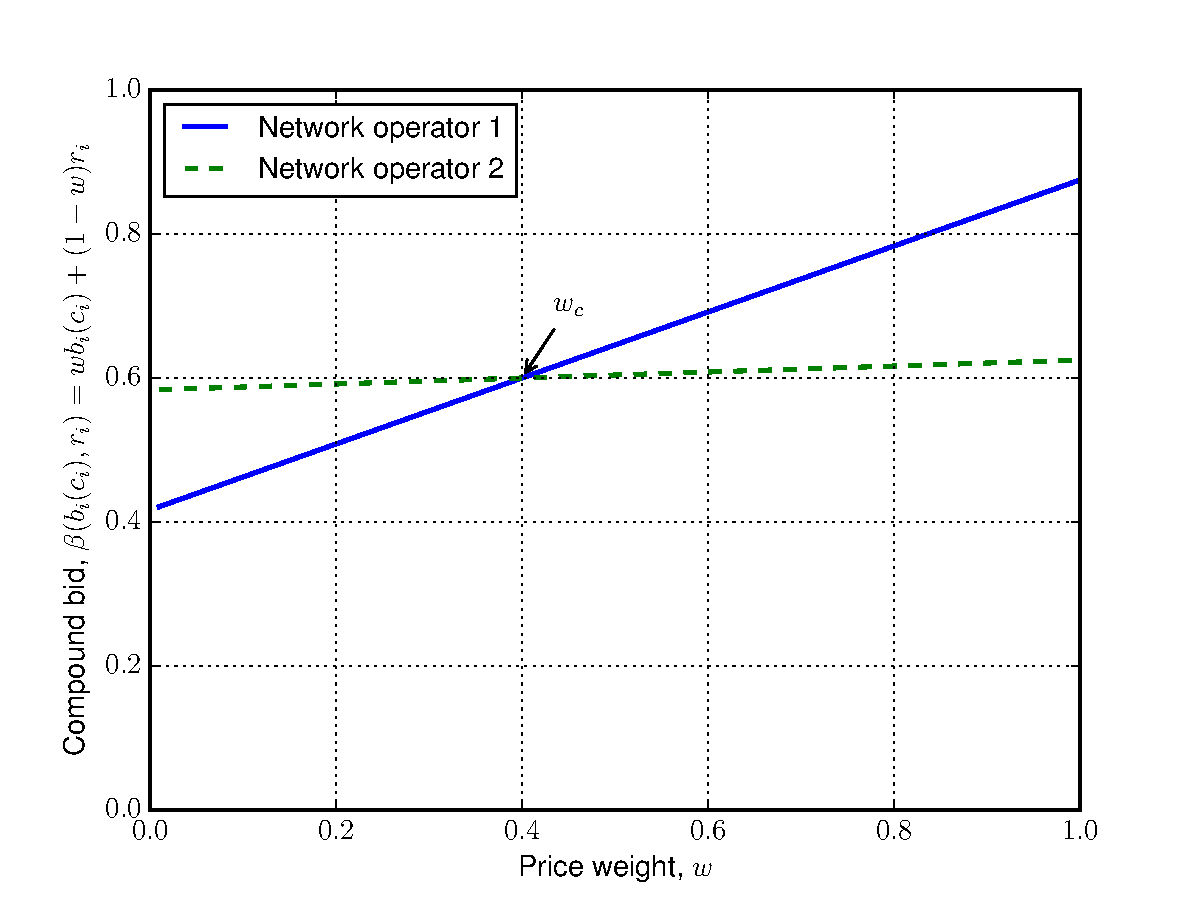
\includegraphics[width=\figsize]{Direct/Figures/pincomplete_bids_uc}
	\caption{Compound bid plotted against the price weight}
	\label{fig:pincomplete_bids_uc_direct}
	\vspace{10mm}
	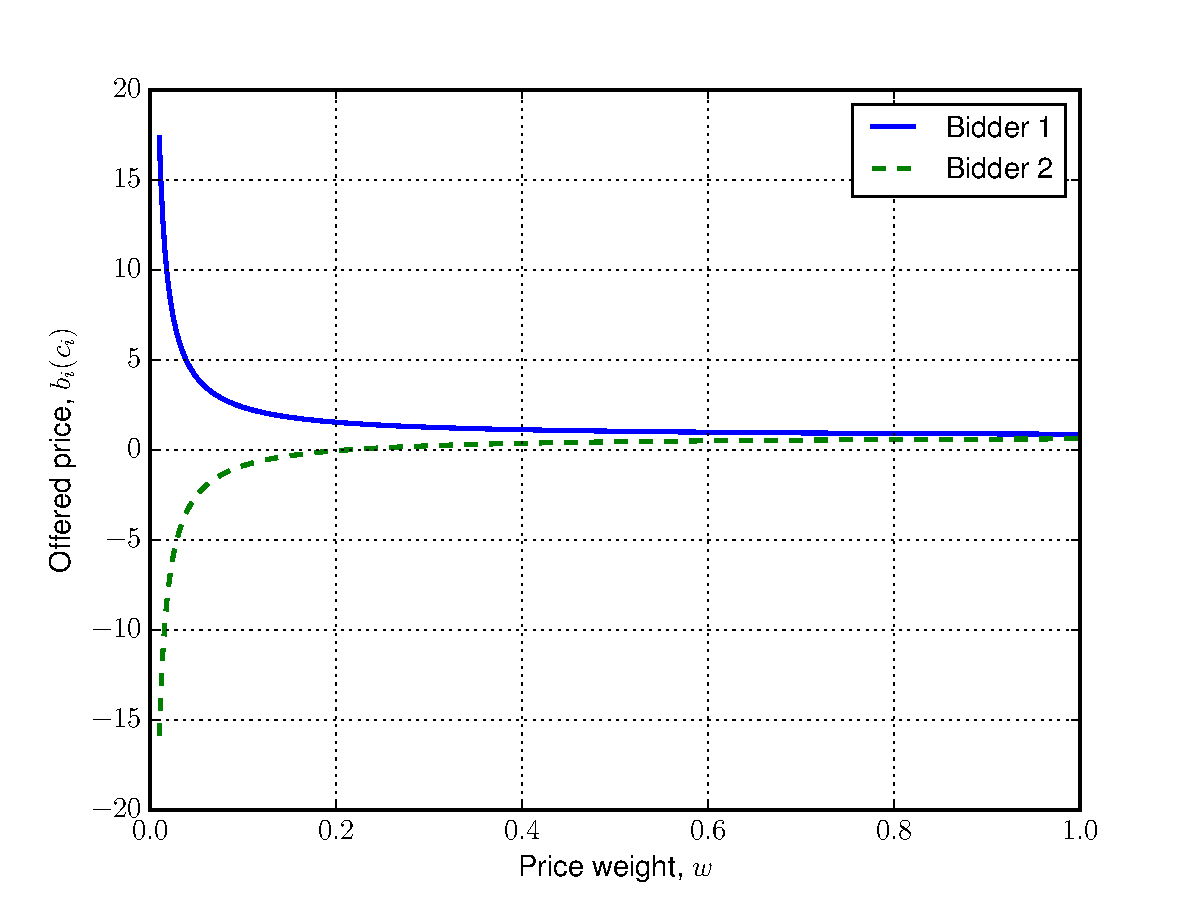
\includegraphics[width=\figsize]{Direct/Figures/pincomplete_prices_uc}
	\caption{Offered prices (bids) plotted against the price weight}
	\label{fig:pincomplete_prices_uc_direct}
\end{figure}

By way of example, Table~\ref{tab:pcomp_direct} depicts a particular set of cost-reputation pairs of two network operators. Figure~\ref{fig:pincomplete_bids_uc_direct} shows the value of the compound bid, $\beta$, for different values of $w$ for both network operators, while Figure~\ref{fig:pincomplete_prices_uc_direct} depicts the value of the monetary bid (or offered price), $b_i$, for different values of $w$ for both network operators. The numerical data in Table~\ref{tab:pcomp_direct} suggests that network operator 2 should be the winner for the values of $w\rightarrow 1$ since network operator 2's cost is strictly lower than that of their opponent's. On the other hand, network operator 1 should be winner for the values of $w\rightarrow 0$ since network operator 1's reputation rating is strictly lower than that of their opponent's (which implies that network operator 1's reputation is in fact strictly higher than that of their opponent's). This prediction agrees with the numerical output shown in Figure~\ref{fig:pincomplete_bids_uc_direct}. Let $w_c$ denote the value of $w$ for which an intersection between the compound bids of both network operators occurs (if it exists). In Figure~\ref{fig:pincomplete_bids_uc_direct}, $w_c=0.4$. Hence, network operator 2 wins the auction for the values of $w\in(w_c,1]$, while network operator 1 for the values of $w\in[0,w_c)$. Note, moreover, that network operator 2 bids below their cost for values of $w<w_c$ (see Figure~\ref{fig:pincomplete_prices_uc_direct}). However, this does not necessarily disqualify the equilibrium bidding strategies given by Equations~\eqref{eq:pcomp_equi_bidding_str_1_direct}~and~\eqref{eq:pcomp_equi_bidding_str_2_direct}. The following observations show why. Firstly,
\begin{proposition}
\label{prop:pcomp_negative_bids_direct}
Suppose both network operators bid according to $b_i$ bidding strategies in Equations~\eqref{eq:pcomp_equi_bidding_str_1_direct}~and~\eqref{eq:pcomp_equi_bidding_str_2_direct}. Then they are guaranteed nonnegative profit in case of winning (or a draw).
\end{proposition}
\noindent Even though the prediction suggests that one of the network operators may bid negatively, they will not win the auction, and hence, are guaranteed profit at worst equal to zero.

Secondly, let $(\mathbf{Q},\mathbf{M})$ be the direct mechanism induced by the equilibrium bidding strategies, $b_i$, in Equations~\eqref{eq:pcomp_equi_bidding_str_1_direct}~and~\eqref{eq:pcomp_equi_bidding_str_2_direct} where $\mathbf{Q}=(Q_1,Q_2)$ and $\mathbf{M}=(M_1,M_2)$. Here, $Q_i$ represents the allocation rule for each network operator $i\in\{1, 2\}$ defined by
\begin{equation}
	\label{eq:pcomp_allocation_rule_1_direct}
	Q_1(c_1,c_2) =
	\left\{
	\begin{array}{l l}
		1 &\text{if } \beta(b_1(c_1),r_1) < \beta(b_2(c_2),r_2),\\
		\frac{1}{2} &\text{if } \beta(b_1(c_1),r_1) = \beta(b_2(c_2),r_2),\\
		0 &\text{otherwise},
	\end{array}
	\right.
\end{equation}
for network operator 1, and
\begin{equation}
	\label{eq:pcomp_allocation_rule_2_direct}
	Q_2(c_1,c_2) =
	\left\{
	\begin{array}{l l}
		1 &\text{if } \beta(b_2(c_2),r_2) < \beta(b_1(c_1),r_1),\\
		\frac{1}{2} &\text{if } \beta(b_2(c_2),r_2) = \beta(b_1(c_1),r_1),\\
		0 &\text{otherwise},
	\end{array}
	\right.
\end{equation}
for network operator 2. $M_i$ for all $i\in\{1,2\}$, on the other hand, denotes the payment rule, and is defined by
\begin{equation}
	\label{eq:pcomp_payment_rule_1_direct}
	M_1(c_1,c_2) = Q_1(c_1,c_2)b_1(c_1)
\end{equation}
for network operator 1, and
\begin{equation}
	\label{eq:pcomp_payment_rule_2_direct}
	M_2(c_1,c_2) = Q_2(c_1,c_2)b_2(c_2).
\end{equation}
for network operator 2. Suppose network operator 2 reveals their cost truthfully. The equilibrium payoff function for network operator 1 characterized by cost $c_1$ but revealing $c'_1$ is
\begin{align}
	\tilde{\tilde{u}}_1(c'_1) &= E\left[ M_1(c'_1,C_2) - c_1Q_1(c'_1,C_2) \right]\nonumber \\
	&= E\left[ (b_1(c'_1)-c_1)Q_1(c'_1,C_2) \right]\nonumber \\
	&= E\left[ b_1(c'_1)-c_1 \:\middle\vert\: \beta(b_1(c'_1),r_1) < \beta(b_2(C_2),r_2) \right].
	\label{eq:pcomp_expected_utility_direct}
\end{align}
It turns out that it is in network operator 1's best interest to reveal their cost truthfully as well; i.e., $c'_1=c_1$. Moreover, both network operators cannot be better off by not participating in the auction; i.e., their equilibrium payoff function is nonnegative, $\tilde{\tilde{u}}_i(c_i)\ge 0$ for all $i\in\{1,2\}$. Formally,
\begin{proposition}
\label{prop:pcomp_direct_mechanism_direct}
The direct mechanism $(\mathbf{Q},\mathbf{M})$ where $\mathbf{Q}=(Q_1,Q_2)$ and $\mathbf{M}=(M_1,M_2)$ satisfies both the IC and IR constraints.
\end{proposition}
\noindent This strengthens the fact that even though the network operators may bid negatively, the auction is still attractive to them.

Thirdly, suppose that economic agents are computers who bid on behalf of the network operators. This assumption is reasonable since there currently are estimated 6.1 billion mobile subscribers around the world \cite{Ericsson2011}. In other words, bidding on a per call basis would have to be automated by the network operators in order to make the process manageable. One way of achieving such an automation would be to utilise the concept of a direct mechanism. In a direct mechanism, economic agents submit their costs (which need not be truthful) directly to the mechanism which then computes the bids and chooses the winner on their behalf. By the Revelation Principle, for every mechanism and an equilibrium for that mechanism, there exists an incentive compatible direct mechanism which yields the same outcomes as in the given equilibrium of the original mechanism (see Section~\ref{sub:mechanism_design_theory_notation}, Appendix~\ref{cha:notation} for the definition of the Revelation Principle). In this case, the direct mechanism $(\mathbf{Q},\mathbf{M})$ is the direct representation of the DMP variant of an FPA. Since it is incentive compatible, economic agents will not lie about their costs. Since it is individually rational, they will find it beneficial to participate in the mechanism. Therefore, the possibility of one of the network operators bidding below their cost or negatively will not matter to any of the network operators and will not lead to an outcome in which the service is sold for a negative price.
% subsubsection incomplete_information_n_2 (end)
% subsection direct_restricted_case_n_2_ (end)

\section{Summary} % (fold)
\label{sec:summary_direct}
In this chapter, game-theoretical model for the DMP network selection mechanism was formally defined. \annotate{C4.11}{Several simplifying assumptions were made in order to keep the analysis mathematically tractable. For example, network operators and the buyer are risk neutral, and the buyer does not have any budget constraints. Despite the fact that those assumptions are not entirely representative of the reality, following in the footsteps of von Neumann and Morgenstern~\cite{VonNeumann2004}, the mathematical theory should be rigorous and developed gradually. Therefore, the simplifying assumptions made in this chapter serve as a starting point for the rigorous, gradual development of the theory of operation of the DMP network selection mechanism before it can embark on capturing the reality to a high degree.}

This chapter further demonstrated that for the price weight of $w=1$, and equal reputation ratings for all network operators, $r_i=r_j$ for all $i\neq j$, the DMP auction reduces to the standard, symmetric FPA (Proposition~\ref{prop:special_case_w_1_direct} and Corollary~\ref{cor:special_case_r_i_r_j_direct}). \annotate{C4.11}{In this case, the abundance of theoretical results and economic insight from the auction literature applies found, for example, in Krishna~\cite{Krishna10}. For the price weight of $w=0$, however, it was shown that the network operators would engage in abnormally high bidding (Proposition~\ref{prop:special_case_w_0_direct}). Hence, charging the buyer the maximum they are prepared to pay for the service. While this result sounds like a potential design flaw in the DMP network selection mechanism, in reality, the buyers will necessarily be budget constrained and therefore, abnormally high bidding of the network operators will translate into charging the buyers a premium price for the service that is within the limits of their respective budgets.}

Finally, the chapter concluded with the specification of an analytical solution to the restricted case of two network operators $n=2$ (Proposition~\ref{prop:pcomp_equi_bidding_str_direct}). The solution is suboptimal in the sense that the derived equilibrium bidding strategies permit the network operators to bid negatively. \annotate{C4.11}{In the view of game theory, this would imply that the network operators are not rational decision-makers. However, it was also shown that negative bidding does not lead to negative profit for either network operator (Proposition~\ref{prop:pcomp_negative_bids_direct}). Concurrently, it was proved that the network operators would not find it beneficial not to participate in the auction if they were to bid according to the strategies summarised in Proposition~\ref{prop:pcomp_equi_bidding_str_direct} (Proposition~\ref{prop:pcomp_direct_mechanism_direct}). It should further be noted that the real behaviour of the network operators might be dictated by the need to secure the contract with the subscriber first and foremost, and hence, lead to negative bidding; a strategy akin to the ``loss leader'' pricing strategy. However, since the ultimate aim of this thesis is to gradually develop rigorous theory of operation of the DMP auction, it is assumed throughout this thesis that network operators will bid at least their cost.}
% section summary_direct (end)
% chapter selling_mechanism_in_the_digital_marketplace (end)
